%\documentclass{article}
% 这里是导言区
%Hello, world!

\documentclass{article}
\title{Sheer}
\author{WingDust}

\usepackage{tikz}  
\usetikzlibrary{positioning,shapes.geometric,arrows.meta}%画箭头用的包


\begin{document} 
\maketitle
Sheer
\section{Sheer}
%
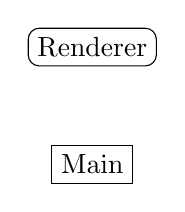
\begin{tikzpicture}
  \node[draw,rounded corners] (start) {Renderer};
  \node[draw,below=of start] (step 1) {Main};
  
%  \draw[->] (0,0)--(7,0);
%  \draw[->] (0,0)--(0,7); %箭头线
%
%  \draw[red] (2,1) -| (1,2);%直角1
%  \draw[blue] (2,1)|-(1,2);%直角2
%  \draw[green] (2,2) circle (1);%圆:圆心、半径
%  \draw[black] (4,4) ellipse (1 and 3);%椭圆:短、长半轴
%  \draw[yellow] (3,3) rectangle (4,1);%矩形
%  \draw[orange] (0,0) -- (2,1-|1,2);%找到垂点并与(0,0)连线
%  \draw[purple] (0,1)--(1,1.5)--(0,2)--cycle  %封闭的线段
%  (0,2)--(1,3);%不加分号的连写
\end{tikzpicture} 

\end{document}